\documentclass{beamer}
% Copyright 2015 by Do Phan Thuan

% Loại mẫu slice
%\usetheme{AnnArbor}
%\usetheme{Antibes}
\usetheme{Boadilla}
%\usetheme{CambridgeUS}
%\usetheme{Hannover}

% Ký tự tiếng Việt
\usepackage[utf8]{vietnam}
\usepackage[utf8]{inputenc}
% Công thức toán
\usepackage{amsmath,amsthm,amssymb,epsfig}
% Chèn ảnh
\usepackage{graphicx}
% Chèn đường dẫn 
\usepackage{url}

% Vẽ đồ thị
\usepackage{pgfplots}

% Insert code
\usepackage{listings}
\lstset{language=C++,
   %keywords={break,case,catch,continue,else,elseif,end,for,function,
   %   global,if,otherwise,persistent,return,switch,try,while},
   basicstyle=\ttfamily,
   keywordstyle=\color{blue},
   commentstyle=\color{red},
   stringstyle=\color{dkgreen},
   frame=lrtb,
   %frame=5 pt,
   numbers=left,
   numberstyle=\tiny\color{gray},
   stepnumber=1,
   numbersep=10pt,
   backgroundcolor=\color{white},
   tabsize=4,
   showspaces=false,
   showstringspaces=false}
% Tô mầu cho bảng
\usepackage{colortbl}


\usepackage{color}

\definecolor{dkgreen}{rgb}{0,0.6,0}
\definecolor{gray}{rgb}{0.5,0.5,0.5}
\definecolor{mauve}{rgb}{0.58,0,0.82}
  
\definecolor{Xanh}{rgb}{0,0.5,1}
\definecolor{Do}{rgb}{1,0.25,0}
\definecolor{Vang}{rgb}{1,1,0}
\definecolor{Datroi}{rgb}{0,0,1}
% Vẽ hình


% multirow
\usepackage{multirow}

\usepackage{pbox}

% Tô mầu cho bảng
\usepackage{colortbl}
\definecolor{Xanh}{rgb}{0,0.5,1}
\definecolor{Do}{rgb}{1,0.25,0}
\definecolor{Vang}{rgb}{1,1,0}
\definecolor{Datroi}{rgb}{0,0,1}

% Một vài ký hiệu thường dùng
\def\R{{\mathbb R}}
\def\N{{\mathbb N}}
\def\X{{\mathcal X}}
\def\Y{{\mathcal Y}}
\def\F{{\mathcal F}}
\def\P{{\mathcal P}}
\def\E{{\mathbb E}}
\def\I{{\mathbb I}}
\def\sign{{\rm sign}}

% Xác định khoảng dãn trong bảng
%\renewcommand\arraystretch{1.6}

% a few macros
\newcommand{\bi}{\begin{itemize}}
\newcommand{\ei}{\end{itemize}}
\newcommand{\ig}{\includegraphics}
\newcommand{\subt}[1]{{\footnotesize \color{subtitle} {#1}}}

% named colors
\definecolor{offwhite}{RGB}{249,242,215}
\definecolor{foreground}{RGB}{255,255,255}
\definecolor{background}{RGB}{24,24,24}
\definecolor{title}{RGB}{107,174,214}
\definecolor{gray}{RGB}{155,155,155}
\definecolor{subtitle}{RGB}{102,255,204}
\definecolor{hilight}{RGB}{22,155,104}
\definecolor{vhilight}{RGB}{255,111,207}
\definecolor{lolight}{RGB}{155,155,155}
%\definecolor{green}{RGB}{125,250,125}

% Minted
%\usepackage{minted}
%\usemintedstyle{monokai}
%\newminted{cpp}{fontsize=\footnotesize}

% Graph styles
\tikzstyle{vertex}=[circle,fill=black!50,minimum size=15pt,inner sep=0pt, font=\small]
\tikzstyle{selected vertex} = [vertex, fill=red!24]
\tikzstyle{edge} = [draw,thick,-]
\tikzstyle{dedge} = [draw,thick,->]
\tikzstyle{weight} = [font=\scriptsize,pos=0.5]
\tikzstyle{selected edge} = [draw,line width=2pt,-,red!50]
\tikzstyle{ignored edge} = [draw,line width=5pt,-,black!20]

%gets rid of bottom navigation bars
\setbeamertemplate{footline}[frame number]{}

%gets rid of bottom navigation symbols
%\setbeamertemplate{navigation symbols}{}

%gets rid of footer
%will override 'frame number' instruction above
%comment out to revert to previous/default definitions
%\setbeamertemplate{footline}{}

% Tác giả, Tiêu đề, vân vân
\title[]{{\huge \bf Hệ gợi ý}\\
  }

\author[]{
Nguyễn Tuấn Đạt\\% \inst{1} 
Đặng Quang Trung\\
}

\institute[]{
%\inst{1}% 
}

\logo{
\includegraphics[scale=0.05]{hust.jpg} \vspace{220pt}}

\begin{document}

\begin{frame}
\titlepage
\end{frame}

\begin{frame}{Nội dung}
\tableofcontents
\end{frame}
\section{Mô tả dữ liệu}
%\section{Xử lý dữ liệu}
%\section{Các phương pháp sử dụng}
%\section{Đánh giá các phương pháp}
%\section{Kết quả}
\begin{frame}{Mô tả dữ liệu}
\textbf{Giới thiệu bộ dữ liệu}
\bi
\item Bộ dữ liệu: ml-20m ( size: 190MB ).
\item Download:\textbf{ \url{http://grouplens.org/datasets/movielens/}}.
\item Bộ dữ liệu mô tả đánh giá 1 - 5 sao phim từ MovieLens.
\item Bộ dữ liệu chứa:
\bi
\item 20000263 rating và 465564 tag của 27278 bộ phim.
\item Dữ liệu đươc tạo bởi 138493  users.
\ei
\item Các users được thu thập ngẫu nhiên. Tất cả users đã đánh giá ít nhất 20 bộ phim.
\item Các file dữ liệu chứa trong 6 tập, genome-scores.csv, genome-tags.csv, links.csv, movies.csv, ratings.csv và tags.csv. 
\bi
\item Các file đã sử dụng: movies.csv và ratings.csv.
\ei
\ei
\end{frame}
\begin{frame}{Mô tả dữ liệu}
\bi
\item Cấu trúc file dữ liệu ratings:
\bi
\item Tất cả đánh giá của người dùng điều chứa trong file ratings.csv
\item Mỗi dòng của file sau dòng header có định dạng\\( userId,movieId,rating,timestamp ).
\item Các rating thực hiện trên thang điểm 5 sao, với gia số ( 0.5 sao - 5.0 sao ).
\ei
\item Cấu trúc file dữ liệu Movies:
\bi
\item Thông tin của các movies chứa trong file moives.csv.
\item Mỗi dòng sau dòng header có định dạng (movieId,title,genres).
\item Genres là danh sách thể loại được lựa chọn: Action, Adventure, Animation , Children's, Comedy, Crime, Documentary, Drama, Fantasy, Film-Noir, Horror, Musical, Mystery, Romance, Sci-Fi, Thriller, War, Western, (no genres listed)
\ei
\ei
\end{frame}

\section{Xử lý dữ liệu}
\begin{frame}{Xử lý dữ liệu}
\begin{itemize}
\item Sử dụng Java để xử lý dữ liệu ban đầu(chuẩn hóa dữ liệu). Các file sử dụng gồm có: ratings.csv, movies.csv.
\item File ratings.csv
\bi 
\item Đưa ra file biểu diễn theo định dạng ( userId,movieId,rating ). 
\item File biểu diễn mà trận rating của các user.
\ei
\item File movies.csv
\bi
\item Đưa ra file dưới dạng ma trận.
\item Hàng biểu diễn cho movie và cột biểu diễn cho danh sách các đặc tính.  
\begin{displaymath}
(i,j) = \left\{ \begin{array}{ll}
1 & \textrm{nếu movie i có đặc tính j}\\
0 & \textrm{nếu movie i ko đặc tính j}\\
\end{array} \right.
\end{displaymath}
\ei
\end{itemize} 
\end{frame}

\section{Các phương pháp sử dụng}

\begin{frame}{Collaborative Filtering}
\color{vhilight}{ Ý tưởng :}
\begin{itemize}
\item Bước 1: Xét người dùng cần gợi ý phim x. Ta tìm tập N người dùng có tập đánh giá phim tương đồng với người dùng x. 
\item Bước 2: Ước lượng đánh giá của người dùng x với những phim mà anh ấy chưa xem bằng cách dựa vào tập N của x. Sau đó, ta đưa ra t phim có ước lượng cao nhất để gợi ý xem cho người dùng x.
\end{itemize} 
\end{frame}
\begin{frame}{Tìm kiếm tập người dùng tương đồng}
Xét một phim i nào đó:
Tính độ tương đồng giữa người dùng x và người dùng y bằng độ đo cosin:
$$sim(x,y)=cos(\overrightarrow{r_x},\overrightarrow{r_y})=\dfrac{\overrightarrow{r_x}\bullet\overrightarrow{r_y}}{||\overrightarrow{r_x}||||\overrightarrow{r_y}||}$$
Với mỗi người dùng ta sẽ chọn ra k người dùng gần với x nhất có đánh giá cho phim i. 
\end{frame}
\begin{frame}{Ước lượng với những phim chưa đánh giá}
Xét người dùng x và bộ phim i $r_xi$ sẽ được ước lượng bằng công thức: 
$$ r_{xi}=\dfrac{\sum_{j\in N(x)} S_{x,j} *r_{ji}}{\sum_{j\in N(x) S_{x,j}}}$$
với : $ S_{xj} $ là độ tương đồng của người dùng x và người dùng j.\\

Ước lượng với trung bình trọng số:
$$r_{xi}=b_{xi}+\dfrac{\sum_{j\in N(i;x)} S_{i,j} \bullet (r_{xj} -b_{xj} }{\sum_{j\in N(i;x)} S_{ij} }$$
Với $$b_{xi}= \mu + b_x + b_i $$ 
\begin{itemize}
\item $\mu$ là trung bình độ lệch 
\item $b_x$ trung bình độ lệch theo người dùng x
\item $b_i$ trung bình độ lệch theo phim i
\end{itemize}

\end{frame}
\begin{frame}{Latent Factor Model}
{\color{vhilight}{ Ý tưởng :}} 
Sử dụng SVD để giảm số chiểu của dữ liệu.
$$R=P*Q^T$$
với Q(item,factor) và P(user,factor);


Ước lượng được tính bằng công thức $$r_{xi}=q_i*p_x$$ 
Hàm đánh giá $$ min_{P,Q} \sum_{i,j\in R} = (R_{ij}-q_j*p_i)^2$$
Để mô hình đúng hơn với S dữ liệu đã bị mất ta thêm vào hàm đánh giá các tham số để mong muốn có kết quả tốt hơn trong việc ước lượng các đánh giá.
$$ min_{P,Q} \sum_{i,j\in R} = (R_{ij}-q_j*p_i)^2+[\lambda_1 \sum_i ||p_i||^2 +\lambda_1 \sum_j ||q_j||^2]$$

\end{frame}
\begin{frame}
Ta sẽ sử dụng SGD để tối thiểu hàm đánh giá:
Ta thu được: \\
Với mỗi $r_{xi}:$
\begin{itemize}
\item $\varepsilon_{xi} =2(r_{xi}-q_i*p_x)$
\item $q_i=q_i+\mu_1(\varepsilon_{xi}*p_x-\lambda_2q_i)$
\item $p_x=p_x+\mu_1(\varepsilon_{xi}*q_i-\lambda_2p_x)$

\end{itemize}
với $\mu_{1,2}$ là tốc độ học 
\end{frame}



\begin{frame}{Content-based}
\textbf{Ý tưởng}: Giới thiệu các movie đến user x với các movie có đặc tính gần với các movie mà user x đã đánh giá cao trước đó.
\bi
\item Mỗi người dùng x sẽ có một vector người dùng.
\begin{figure}[h]
\begin{center}
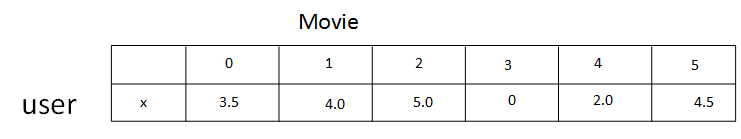
\includegraphics[width =0.7 \textwidth]{img1.png}
\caption{vector người dùng}
\end{center}
\end{figure}
\item Chọn ngưỡng đánh giá rating của người dùng $\alpha$
\begin{displaymath}
(x,i) = \left\{ \begin{array}{ll}
1 & \textrm{nếu rating(x,i) $\geq \alpha $}\\
-1 & \textrm{nếu rating(x,i) $\le \alpha$ }\\
\end{array} \right.
\end{displaymath}
\ei
\end{frame}
\begin{frame}{Content-based}
\bi
\item $\alpha = 4.0$ Ta có vector người dùng
\begin{figure}[h]
\begin{center}
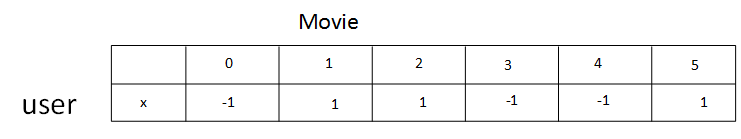
\includegraphics[width =0.7 \textwidth]{img2.png}
\caption{vector người dùng sau khi đánh giá}
\end{center}
\end{figure}
\item Tìm đặc tính của user ta thực hiện:
\bi
\item  $V_{feature}  =  V_{user} * M_{movie}$. \\
Trong đó: $V_{feature}$ vector đặc tính người dùng, $V_{user}$ vector người dùng, $M_{movie}$ ma trận movie và các đặc tính.
\ei
\ei
\end{frame}
\begin{frame}{Content-based}
\bi
\item Chuẩn hóa lại $V_{feature}$
\begin{displaymath}
V_{feature}(i) = \left\{ \begin{array}{ll}
1 & \textrm{nếu  $V_{feature}(i) > 0$}\\
0 & \textrm{nếu  $V_{feature}(i) < 0$ }\\
\end{array} \right.
\end{displaymath}
\item Sử dụng độ đo Cosin để tình khoảng cách giữa vector đặc tính của người dùng và movie
\item Gợi ý những movie gần với vector đặc tính của người dùng.
\ei
\end{frame}
\section{Đánh giá các phương pháp}
\begin{frame}{RMSE}
Sử dụng tiêu chuẩn ước lượng:\\
Root Mean Square Error (RMSE): $\sqrt{\dfrac{1}{|R|}\sum_{(i,x)\in R} (\hat{r_{xi}}-r_{xi})^2}$\\
Ước lượng trên chỉ áp dụng được với Collaborative Filtering và Latent Factor Model, Content-base không thể đánh giá theo phương pháp này.
\end{frame}
\section{Kết quả}
\begin{frame}{Thực hiện}
\begin{itemize}
\item Sử dụng Java để tạo ma trận dữ liệu.
\item Sử dụng nén thưa(thư viện Java, Matlab) để nhét toàn bộ tập dữ liệu vào bộ nhớ.
\item Tách lấy 1000 rating làm tập test phần còn lại làm tập train.
\end{itemize}
\end{frame}
\begin{frame}{Collaborative Filtering}
\begin{itemize}

\item Chọn k=5,10 phần tử có độ tương đồng gần nhất.
\item Kết hợp với trung bình trọng số để đoán các rating trong tập test.

\end{itemize}
\end{frame}
\begin{frame}{Latent Factor Model}
\begin{itemize}
\item Chọn số factor=30,50,100 (30).
\item Lựa chọn các tham số $\mu \approx 0.0002 (0.0001)$ .
\item Chọn $\lambda \approx 0.1 (0.02)$ .
\item Sử dụng Stochastic Gradient Descent.
\end{itemize}

\end{frame}
\begin{frame}{Kết quả}
Dự đoán trên 1000 tập rating ngẫu nhiên
\begin{itemize}
\item Collaborative Filtering(k=5) : 1.13
\item Latent Factor Model(Matlab SVD: 1.4406)
\item Latent Factor Model($\lambda_1=\lambda_2=0.002, SGD)$ : 3.5(cũ) ?? (update 1.1361)
\end{itemize}

\end{frame}
\begin{frame}{Cảm ơn thầy và các bạn đã lắng nghe}
\includegraphics[scale=0.6]{thanks.jpg}
\end{frame}
\begin{frame}{Tài liệu tham khảo}
\section*{Tài liệu tham khảo}
\begin{itemize}
\item Slide Datamining Stanford
\end{itemize}
\end{frame}
\end{document}